\documentclass[11pt]{article}

\usepackage{amsmath}
\usepackage{amsxtra}
\usepackage{amsfonts}
\usepackage{amssymb}
\usepackage{amsthm}
\usepackage{graphicx}
\usepackage{mathtools}
\usepackage{dsfont}
\usepackage{hyperref}

\graphicspath{ {/Users/andrew/hw/math191k/figures/}}

\usepackage[margin=3cm]{geometry}
\newcommand{\eps}{\varepsilon}
\newcommand{\Z}{\mathbb{Z}}
\newcommand{\N}{\mathbb{N}}
\newcommand{\R}{\mathbb{R}}
\newcommand{\Q}{\mathbb{Q}}
\newcommand{\W}{\mathcal{W}}
\newcommand{\U}{\mathcal{U}}
\newcommand{\V}{\mathcal{V}}
\newcommand{\C}{\mathbb{C}}
\newcommand{\K}{\mathcal{K}}

\newcommand{\set}[1]{\{ #1 \}}
\newcommand{\gen}[1]{\left\langle #1 \right\rangle}
\newcommand{\floor}[1]{\left\lfloor #1 \right\rfloor}
\newcommand{\abs}[1]{\left| #1 \right|}
\renewcommand{\phi}{\varphi}
\renewcommand{\Re}{\operatorname{Re}}
\renewcommand{\Im}{\operatorname{Im}}
\newcommand{\conj}[1]{\mkern 1.5mu\overline{\mkern-1.5mu#1\mkern-1.5mu}\mkern 1.5mu}
\newcommand{\defeq}{\vcentcolon=}
\newcommand{\identity}{\mathds{1}}

\DeclareMathOperator{\im}{im}
\DeclareMathOperator{\res}{Res}
\DeclareMathOperator{\Arg}{Arg}
\DeclareMathOperator{\parg}{arg}
\DeclareMathOperator{\Log}{Log}

\theoremstyle{plain}
\newtheorem{thm}{Theorem}

\theoremstyle{definition}
\newtheorem{recall}{Recall}
\newtheorem{remark}{Remark}
\newtheorem{definition}{Definition}
\newtheorem{prop}{Proposition}
\newtheorem{cor}{Corollary}
\newtheorem{lemma}{Lemma}
\newtheorem{ex}{Example}
\newtheorem{claim}{Claim}
\newtheorem{exercise}{Exercise}
\newtheorem{notation}{Notation}
\newtheorem{question}{Question}

\title{Lectures notes on knot theory}
\author{Andrew Berger}

\begin{document}
\maketitle

\clearpage

\tableofcontents


\clearpage
\section{Disclaimer}

Caution - these lecture notes have not been proofread and may contain errors, due to either the lecturer or the scribe. Please send any corrections or suggestions to \href{mailto:andbberger@berkeley.edu}{andbberger@berkeley.edu}

\clearpage

\section{1/19/16: Introduction + Motivation}

Start with a joke: ``Applied Math majors may have misread the course title''

\bigskip
- hand out syllabus \& table of knots

- administration \& logistics

- ``idea'' of class structure

- find out about class (their backgrounds \& interests)

\bigskip
- introduce some material:

1) knots come from real life: tie ends of string together

- unknots

- simplest possible knot = trefoil

2) not everything is a circle

- want to distinguish them

- knot complements

- techniques?

3) links ? can be complicated while component knots simple

4) crossings / deformations

- swap crossings of trefoil to get its mirror (interesting fact: they're not equivalent!)

5) usefulness:

- want to know when objects are knotted

- get all 3-dimensional spaces

- applications to physics

\clearpage
\section{1/21/16: 2nd class}

\subsection{Logistical things}

Talk to Chris if you're uncomfortable with group theory. There are going to be two projects (long and short) - we'll start breaking up in to groups to work on those starting the second week of February.

\subsection{Minimal introduction to point-set topology}

Just to set terms and notation for future reference.


\begin{definition}
  Some miscellaneous definitions:

  \begin{itemize}
  \item $\R^n \defeq \R \oplus \ldots \oplus \R$
  \item $B^n = \set{x \in \R^n | \abs{x} \leq 1}$ note that in general this includes the boundary (which we call $\partial B^n = S^{n -1}$, the $n - 1$ sphere)
  \item There are many ways to get the inclusion $\R^m \subseteq \R^n$ for $m \leq n$, as a convention just take the first $m$ elements from $\R^n$
  \end{itemize}
\end{definition}


\begin{remark}
  The (closed) line and circle are the only 1-dimensional topological spaces (once we have defined appropriate notions of equivalence). More on this later
\end{remark}


\begin{definition}[Homeomorphism]

  We say that $f$ is a \emph{homeomorphism} if it is a bicontinuous bijection (both $f$ and its inverse are continuous). Two topological spaces $X, Y$ are homeomorphic
  if there exists $f: X \to Y$ a homeomorphism, denoted $X \cong Y$
\end{definition}

\begin{remark}
  Given $X, Y$ topological spaces and $f: X \to Y$ a homeomorphism we can `pull' the notion of openness in $X$ into
  a notion of openess in $Y$: $A \subseteq Y$ is open if $f^{-1}(A)$ is open in $X$
\end{remark}



\begin{ex}
  Examples of homeomorphisms
  \begin{itemize}
  \item $(0, 1) \cong \R$. As an exercise find the homeomorphism that is witness to this fact (hint: use an arctangent)
  \item A square in the plane is homeomorphic to a circle in the plane
  \item $\R^n \not \cong \R^m$ for $n \neq m$: dimension is invariant under homeomorphism. This is a deep result
    that is supposed to be hard to prove
  \end{itemize}
\end{ex}


\begin{definition}[Knot]
  A knot is a one-dimensional subset of $\R^3$ that is homeomorphic to $S^1$.

  We can specify a knot $K$ by specifying an embedding (smooth injective) $f: S^1 \to R^3$
  so that $K = f(S^1)$. For $f$ to be smooth, all of its derivatives must exist.
\end{definition}


\begin{ex}
  Examples of embeddings specifying knots
  \begin{itemize}
  \item $f = \mathds{1}$ (abuse of notation here) specifies a circle
  \item The infinite non-knot example we looked at yesterday fails to be a knot because the derivative does not exist
    at the limit point
  \end{itemize}
\end{ex}


\begin{definition}[Link]
  Given a collection of knots $\set{K_i}$, we define a link $L = \bigcup_i K_i$ (disjoint union)
\end{definition}

The study of links is different from the study of knots, due to ``linking behavior''. Roughly speaking: knots can be very complicated as well their disjoint unions, but moreover, links can get very complicated while their connected components may all be unknots.

\subsection{Equivalence of knots}

Our word for equivalence of knots is ambient isotopy. This refers to the fact that the homeomorphism that is witness
to the equivalence of the knots acts on the ambient space the knots lives and not only on the knot itself.




\begin{definition}[Equivalence of knots]
  For $K_1, K_2$ knots, we say that $K_1 \cong_{isotopic} K_2$
  if there exists a homeomorphism $f: \R^3 \to \R^3$ such that $f(K_1) = K_2$.

  More precisely we require that there exists a 1-parameter family $\set{f_t}_{0 \leq t \leq 1}$ of smooth homeomorphisms such that $f_0 = \identity$ and $f_1 = f$. In particular, we cannot have an isotopy that shrinks a knot to a point.

  This aligns pleasingly for the intuitive notion that knots are equal when they can be deformed to each other:
  $f$ here is just the global deformation.
\end{definition}

\begin{remark}
  Careful about the notation here: $K_1 \cong K_2 \cong S_1$ holds for any knots $K_1, K_2$
\end{remark}


\begin{definition}[Knotted]
  We say that a knot $K$ is \emph{knotted} if $K \not \cong_{isotopic} S_1$
\end{definition}


\begin{definition}[Planar diagram of $K$]
  When we visualize knots we make some projection $\R^3 \to \R^2$ (with defined coordinate system). The na\"ive projection that discards information about the crossings
  is called the universe and is not necessarily unique. The planar diagram is this projection with crossing information captured.

\end{definition}

\begin{ex}
Examples of invariants (under equivaence)
\begin{itemize}
  \item Dimension is an invariant of isotopy
  \item The crossing number is the minimal number of crossings in a given diagram
\end{itemize}
\end{ex}

\subsection{Reidemeister moves}

What does an isotopy mean for planar diagrams? The famous Reidemeister moves


\begin{definition}[Reidemeister moves]

  \begin{enumerate} Refer to figure~\ref{fig:reidemeister}
  \item R0: You can straighten wiggly lines
  \item R1: You can undo twists
  \item R2: You can seperate underpasses (that don't intersect)
  \item R3: You can move a line behind an intersection across the intersection
  \end{enumerate}
\end{definition}


\begin{figure}[h]
  \centering
  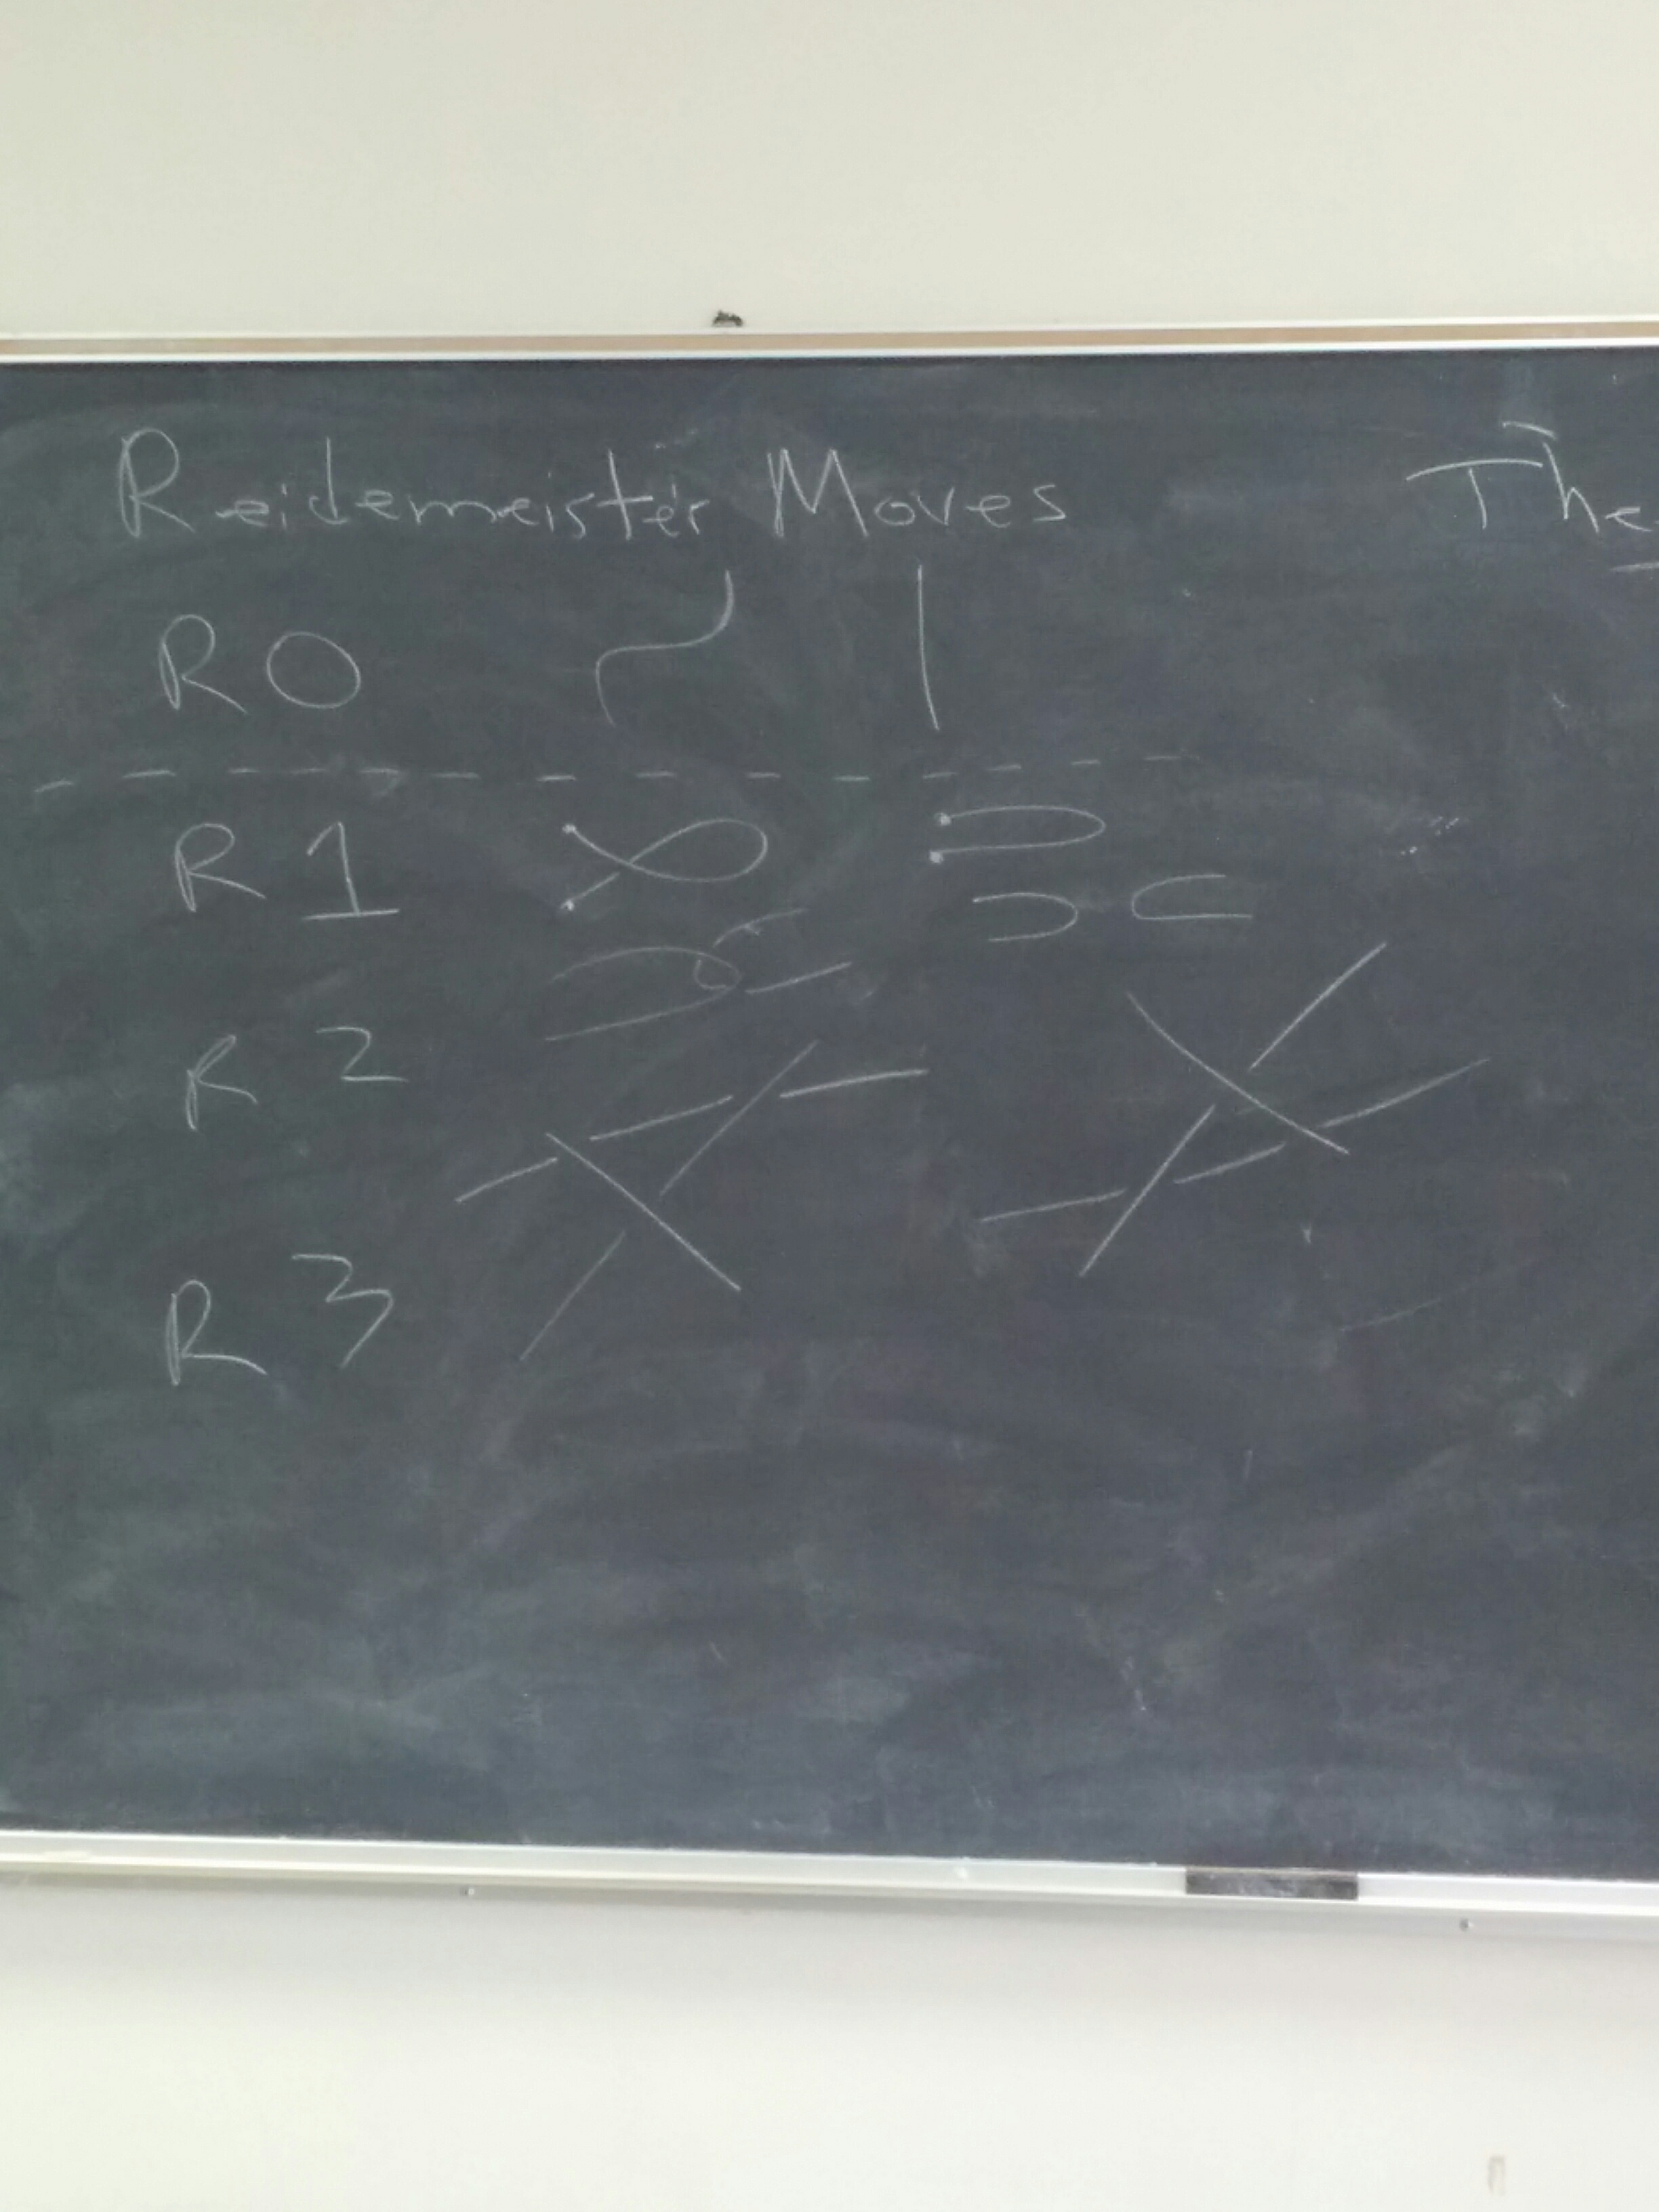
\includegraphics[width=\textwidth]{reidemeister.jpg}
  \caption{Sketch of allowed Reidemeister moves}\label{fig:reidemeister}
\end{figure}


\begin{thm}
$K_1 \cong_{isotopic} K_2$ iff their diagrams can be obtained from each other using the Reidemeister moves
\end{thm}

Wherein Chris struggles to draw a trefoil.

\begin{exercise}
  \begin{enumerate}
    \item Show that the figure eight knot is equivalent to its mirror.
    \item Take your favorite knot diagram and show that it is equivalent to the diagram obtained as follows: Take an arc on the left-most side of your diagram, put a twist in it and then pull it all over to the right side of the diagram. (The point of this exercise is to give an abstract proof of equivalence using Reidemeister moves without worrying about the explicit diagram.)
    \item Show that an unknot with a couple of loops is equivalent to the unknot \emph{without} using R1
  \end{enumerate}
\end{exercise}


\clearpage
\section{1/26/16: recap of the last lecture}

\subsection{Recap of last lecture}

What does it mean to be a knot? To be knotted?


\begin{recall}
  Recall that a knot $K$ is a subset of $\R^3$ that is homeomorphic to $S^1$.

  We could equally as well have defined a knot to be the image $f(S^1)$ of a smooth embedding $f: S^1 \to \R^3$.
\end{recall}


\begin{notation}
  Let's fix our notation for ambient isotopy (the kind that captures a notion of knottedness) and homeomorphism (under which all knots are equivalent), being very careful to distinguish between them.
  \begin{itemize}
  \item For $K_1, K_2$ knots that are equivalently knotted (or isotopic) and write $K_1 \cong K_2$
  \item We write homeomorphism with $\approx$. For instance, all knots $K$ are homeomorphic to $S^1$, $K \approx S^1$
  \end{itemize}
\end{notation}

\subsection{Intro to knot complement}

We expect that the knot complement $\R^3 \setminus K$ should somehow capture the notion of knottedness. Can we formalize that?

`It's not the space itself - it's what the knot is doing in 3-dimensional space that matters, and this theorem captures that precisely'


\begin{thm}[Gordon-Luecke]
  If $\R^3 \setminus K_1 \approx \R^3 \setminus K_2$ then $K_1 \cong K_2$
\end{thm}


\begin{remark}
  The fundamental group sometimes allows us to answer the question `$\R^3 \setminus K_1 \approx \R^3 \setminus K_2$?' and therefore turn this into an algebraic problem.

  Francesca pointed out that the converse of the preceding theorem is easily proved, directly from the definition of equivalence. Do it as an exercise!
\end{remark}

\begin{question}
  Marissa asked: when is a knot equal to its mirror? Chris isn't aware of any general classification results - maybe when the Jones polynomial has palyndromic coefficients.
  Another question: if $K_1 \cong K_2$ is it true that $K_1^\ast \cong K_2^\ast$ (here $K^\ast$ indicates the knot mirror)
  Yet another question: if $K_1 \cong K_2$ and $K_1 \cong K_1^\ast$ is it true that $K_2 \cong K_2^\ast$? Someone
  pointed out that if you can prove the previous statement, then this statement is easily proved to be true.
\end{question}

\subsection{Hard Unknots}

Chris struggles again to draw a trefoil.

Let's fix a notion of complexity for knot diagrams - we say that the complexity of a diagram is the crossing number of that diagram.

Recall that a knot is equivalent to the unknot if it \emph{has a diagram} with crossing number zero. A natural direction to head in towards proving that the trefoil is not the unknot might be to show that any Reidemiester move can
not decrease the complexity of the trefoil diagram - but one needs to be very careful here as there may be a sequence that increases in complexity for a while before decreasing.

This motivates the concept of hard unknots: unknots that require a sequence of Reidemeister moves increasing the complexity of the diagram before the complexity finally falls to zero.


To begin with let's study a hard unknot called `the culprit' from the paper \emph{Hard Unknots and Collapsing Tangles} (Kauffman, Lambropoulou). Can you see how to untangle this knot?

\clearpage
\section{1/28/16}

Agenda: what sort of invariants; solved problem from last class;
oriented knots, linking numbers, fundamental group of a knot

\subsection{Logistical things}

Start thinking about what you want to do for a project.


\subsection{Question from last time}

If $K \cong J$ does $K^\ast \cong J^\ast$?

One idea is that if $D_K$  and $D_J$ are diagrams for $K, J$, then we can find a sequence of R-moves $\set{R_i}$ transforming $D_K$ to $D_J$. It's easily imagined that if we just `flip' the moves in $\set{R_i}$ then
that new flipped sequence transforms $D_{K^\ast}$ to $D_{J^\ast}$. This idea can be used to prove that $K \cong J \implies K^\ast \cong J^\ast$.

Chris came up with a different proof:

First a false proof:

Fact: $\R^3 \setminus K \approx \R^3 \setminus K^\ast$. So if one na\"ively applies the Gordon-Luecke theorem, they conclude $K \cong K^\ast$, which is obviously false.

What gives here is that the Gordon-Luecke theorem requires that the homeomorphism is orientation-preserving. The map that's witness to the fact that $\R^3 \setminus K \approx \R^3 \setminus K^\ast$ is orientation reversing. Thus
the Gordon-Luecke theorem does not apply.

Let's do a real proof:

\begin{lemma}
  If $K \cong J$ then $K^\ast \cong J^\ast$
\end{lemma}

\begin{proof}
  Suppose that $K,J$ are knots such that $K \cong J$. By the Gordon-Luecke theorem $\R^3 \setminus K \approx \R^3 - J$ in an orientation preserving fashion.

  $\R^3 - K^\ast \approx \R^3 - K$ with an orientation reversing homeomorphism; same for $J$. Now we can easily obtain the desired orientation preserving map that's witness to
  $\R^3 - K^\ast \approx \R^3 - J^\ast$ by the appropriate composition (note here, that the composition of an even number of orientation-reversing maps is orientation-preserving).
\end{proof}

\subsection{Connect sum operation, knot cancelling, prime knots}

\begin{definition}[connect sum]
  This is a general concept from algebraic topology, but for our purpose the connect sum of knots $K$ and $J$ (written $K\#J$) is given
  by cutting knots $K$ and $J$ at some point and pasting them together.
\end{definition}


\begin{remark}
  Is this operation well-defined? In particular, does it matter where we choose to cut and paste the knots together?


  Yes it is, and no it does not. A pictoral proof: if we connected the knots in one place and we want to connect in another we can just slide the knots along each other until we arrive at the desired location.

  One thing that does matter is orientation - if we don't assign an orientation there are two ways to join the arcs together at one location. We can resolve this by giving knots an orientation and making
  $\#$ preserve that.
\end{remark}

Chris refined his technique for drawing the trefoil; it is now foolproof.

\begin{question}
  Let $\K$ be the collection of knots (up to $\cong$). Is $(K, \#)$ a group?


  \begin{itemize}
  \item $K \# 0 \cong K$, so there is an identity element. ($0$ indicates the unknot)
  \item $K_1 \# K_2 \cong K_2 \# K_1$, as can seen by a pictoral proof, so this operation is commutative.
  \item It's associative too (we can attach anywhere and at any time).
  \item Okay, do knot inverses exist? No. Knots cannot be cancelled.
  \end{itemize}
\end{question}

\begin{remark}
In particular, it is not possible that $0 \# 0 \cong K$ with $K$ knotted.
\end{remark}

\begin{thm}
  Knots cannot be cancelled under connect sum
\end{thm}

\begin{proof} This is known as the Mazur-Swindle. \\
  To prove this, we have to expand our notion of knots to include wild knots (those that shrink to a point).

  Suppose that $K \# J \cong 0$. Now construct the infinite connect sum $K \# J \# K \# J \dots$ letting the knots shrink in space
  as the sum goes along so that they occupy a closed topological space\footnote{If we let the knots go off to infinity without shrinking them, then do not form a loop and are not captured by our notion of knots.
  By shrinking them they become wild, but are still homeomorphic to $S^1$}.

  We have that $(K \# J) \# (K \# J) \dots \cong 0$ but $K \# (J \# K) \# (J \# K) \cong K \# 0 \cong K$, and thus are knots must be unknotted to begin with!
\end{proof}


\begin{question}[Unsolved]
  Does $c(K \# J) = c(K) + c(J)$ where $c$ is the minimal crossing number operation.
\end{question}


\begin{definition}[Prime, composite knots]
  $K$ is called composite if it can be given as $K_1 \# K_2 \cong K$ for $K_1 \not \cong 0$ and $K_2 \not \cong 0$.

  Otherwise, $K$ is called prime. 
\end{definition}


\begin{exercise}
  Show that the trefoil and figure 8 knots are prime.
\end{exercise}








\end{document}
